\chapter{Selective DNA sequencing}

\label{kap:selSeq} % id kapitoly pre prikaz ref

In this chapter, we are going to explain what is selective sequencing. We
show what advantages this method brings and then look at the main challenges and
the current state of research in this area.

\section{DNA nanopore sequencing}

\subsection{DNA}

% TODO: pridat zdroj %https://en.wikipedia.org/wiki/Genetics#DNA_sequencing_and_genomics
Genetics is a branch of biology that studies genes, genetic variation, and heredity.
It tries to explain the variability between animals, the source of hereditary diseases, and
other important things that influence our lives. The DNA is the key molecule
that stores biological information in living organisms. It is contained in
almost every living cell. Based on the information from this molecule our cells can reproduce and create copies of
themselves. Nowadays, it is possible to look at the DNA of the organism. This is
one of the strongest tools of genetics as it helps us tell what are the functions
of different parts of DNA by comparing it between organisms and looking at the
consequences of different mutations. DNA stores genetic information in the form of a sequence of
nucleotides. The stored information is defined by their particular order. There are four types of DNA nucleotides:
adenine(A), cytosine(C), guanine(G) and thymine(T). In fact, DNA consists of two long
strings of these nucleotides that together create the DNA molecule. However, these
two strings are connected in a complementary way. If there is A on one string
then on the other one must be T. If there is a C then on the other string we can expect
it's complement G. For the organisms, it means that they can (to some extent) repair
missing nucleotides based on the complement rules. An example of how we can think
of DNA is on \ref{obr:acgt}. From now, we will for simplicity assume that DNA
sequence is a sequence of characters A, C, G, T. This simple representation
is very good as it can be easily represented in the computer. It also stores enough
information so we can recover the other complementary DNA string easily.
The process of obtaining DNA sequence is called \textit{DNA sequencing}.

% TODO: obrazok zdroj https://www.genome.gov/genetics-glossary/acgt

\begin{figure}
\centerline{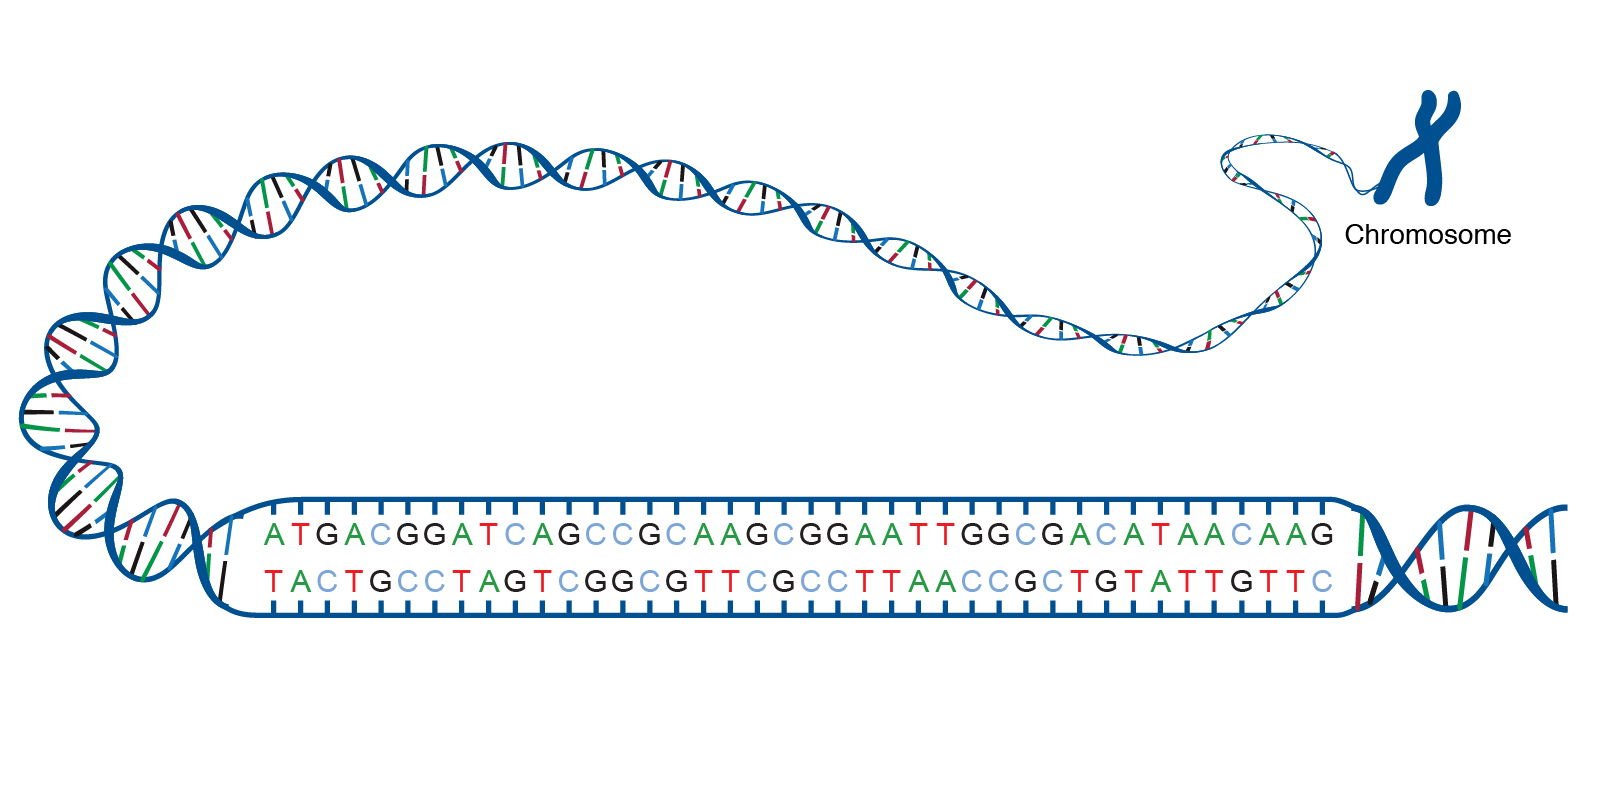
\includegraphics[width=0.7\textwidth, height=0.3\textheight]{images/acgt}}
\caption[DNA]{DNA Molecule}
\label{obr:acgt}
\end{figure}

\subsection{DNA sequencing}

The DNA molecule is very long and processing it whole at once would be very hard.
Single DNA molecule in one cell can reach up to 2 meters when untangled.
%https://www.sciencefocus.com/the-human-body/how-long-is-your-dna/
Thus, it is convenient to broke down the whole DNA molecule into many shorter parts.
This can be done chemically but it brings some problems, especially some of the
DNA molecules could be missed during sequencing so we would lose information about
the corresponding part of DNA. Because of this, we use DNA polymerases to duplicate these shorter DNA sequences
many times so we end up with a mixture containing our DNA molecule, broken into
many duplicated parts. DNA polymerases can stick to the DNA molecule and rebuild the complementary
part which in fact creates a copy of that particular DNA molecule.
Once we have this mixture of shorter DNA molecules we need to sequence individual
parts and then somehow connect them together to obtain the nucleotide string representing
our original DNA molecule.

One of the devices that serve this purpose is MinION\cite{lu2016oxford}. MinION is
a cheap and versatile DNA sequencer with the size of the modern smartphone showed in
\ref{obr:minIon}.

\begin{figure}
\centerline{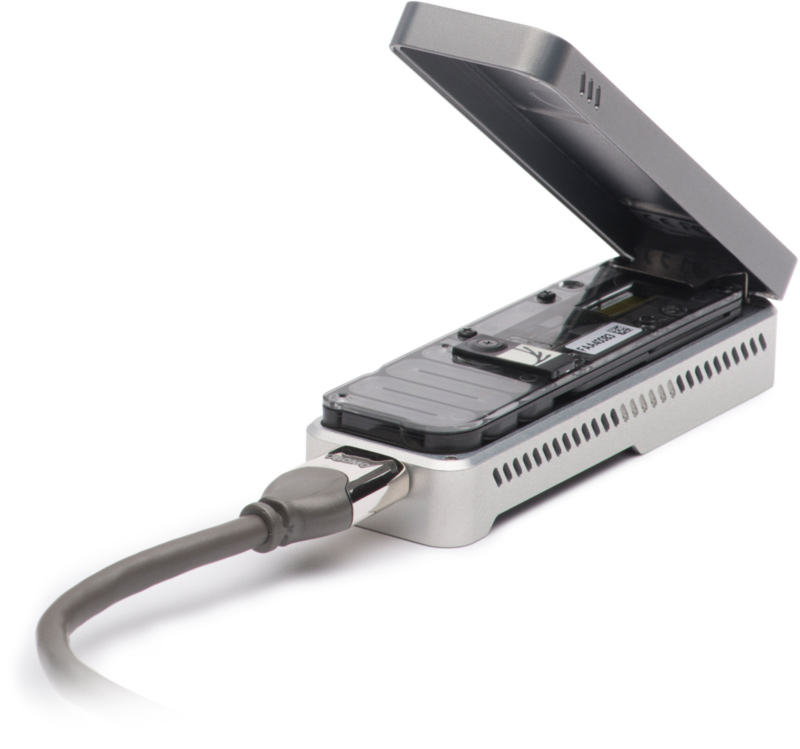
\includegraphics[width=0.7\textwidth, height=0.3\textheight]{images/minion}}
\caption[MinION]{MinION sequencer}
\label{obr:minIon}
\end{figure}

This sequencer consists of an active surface filled with many \textit{nanopores}. A nanopore
is a small hole with an electric current passing through it. When the positive charge
is generated on the other side of the surface negatively charged DNA molecules
will start to pass through the pores. As the molecule of DNA is passing through the pore of
MinION, we can observe changes in the flow of an electric current passing through the pore.
This electric current is measured over the discrete-time and it is called \textit{signal},
\textit{raw signal} or \textit{squiggle}. The example of the squiggle is on figure \ref{obr:minIonCurrent}.

\begin{figure}
\centerline{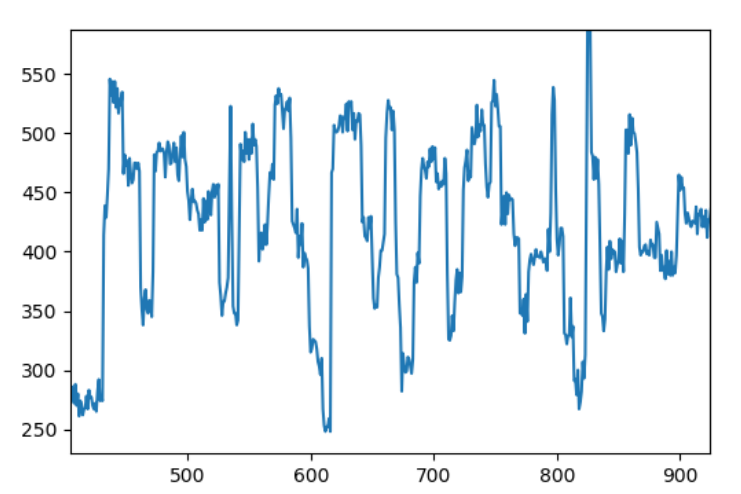
\includegraphics[width=0.7\textwidth, height=0.3\textheight]{images/signal}}
\caption[MinION signal]{Electric current (squiggle) coming from MinION.}
\label{obr:minIonCurrent}
\end{figure}

The MinION version we use for the DNA sequencing process around 400 nucleotides per second
per the nanopore. The value of the current signal is measured around 4000 times per second so it is good to
estimate that one nucleotide produces on average about 10 signals. The signal
generated from the pass of the single DNA molecule through the single pore is called \textit{read}.
One of the advantages of the MinION sequencer is that it produces quite long reads.
The length of the read is stated in kb(kilo-bases) where base corresponds to one nucleotide.
The mean length of the read in some scenarios ranges from 13kb to 20kb. Additionally,
due to fact that MinION has several nanopores it can process multiple DNA molecules in
parallel.

% TODO: https://www.ncbi.nlm.nih.gov/pmc/articles/PMC5793790/

When we obtain the raw signal from the pore, we need to finally convert it into the DNA
sequence. What is crucial for transcription of the signal into the DNA sequence is
that as the molecule of DNA is passing through the pore, only a small
number of nucleotides in the proximity of pore influence the current output signal.
The sequence of $k$ nucleotides is called \textit{k-mer}. An output signal of MinION
is not dependent only on nucleotide currently in the pore but rather by current
3-mer that is present in the proximity of the pore. There are several studies on
how much is signal influenced by more distant nucleotides. However, the version
of MinION we are working with is said to be influenced mainly by the closest 6-mer. 
Usually, with the MinION we are provided a kmer model. It is a list of all possible
$k$-mers for some $k$ that states the mean and standard deviation of a Gaussian
distribution that describes expected signal for the particular $k$-mer.
So from the measurements of signal throughout the time, using a method called base-calling, we can tell how the molecule
of DNA looked like. The early base-calling algorithms tried to split the signal into
\textit{events}. Event is a longer sequence of signals at the roughly same level corresponding
to one particular $k$-mer. From the mapping of the events to particular $k$-mer using
a $k$-mer model they tried to predict what sequence passed through this pore.
Now, the more successful base-calling algorithms are based on recurrent neural
networks. Despite big improvements in the base-calling algorithms, the overall
process of base-calling is quite slow and resource-intensive. 

After the base-calling, we need to join this all base-called reads together to form the
resulting DNA sequence. This is quite hard as the base-calling process is not perfectly
accurate and produces some errors. Thanks to the duplication of the shorter DNA
sequences, we are in most cases able to reconstruct the original DNA string.

\subsection{Selective sequencing}

MinION has a special ability that helps us in certain scenarios. It can reject
DNA molecule that is currently passing through the pore. MinION reverses the molecule’s direction and throws it away.
\textit{Selective sequencing} is the idea that based on the incoming signal, we can tell
if we are interested in sequencing the current DNA molecule. Subsequently, we can decide if we want
to continue or reject this molecule. This happens on-the-fly so we need to make
the decision until the end of the current read.

There are a lot of benefits of selective sequencing. In case we are not interested
in some DNA that we know is contained in our sample, we can use this technique to
reject unwanted DNA molecules. This saves us a lot of time and resources as obtaining
nucleotide sequence from the signal is in some scenarios unnecessary and too
costly process in terms of performance. With selective sequencing, we only have
to further process reads we are interested in.

Let us say we are trying to find an exact type of virus in human blood. We can
reject all human DNA molecules because we are not interested in processing human
DNA. We could also filter positively. So we could say, that we are only
interested in sequencing DNA that produces a signal in some sense similar to our
chosen sample. This all means saving a lot of time and computing power in certain
cases, for example during the disease diagnosis process.

Naturally, there are some drawbacks to selective sequencing. In order to find out
if the currently passing molecule is from human DNA, we have to have some information
about the signal from human DNA beforehand.
This is of course in some sense limiting factor as we need a sample signal from
the species that we want to filter. The other problem is that in the case of misclassifying
some signal as not interesting, we lost information about the corresponding
part of the DNA molecule.

The idea of accessing real time data during the phase of reading the DNA molecules
and rejecting the DNA molecule based on this data is called \textit{Read Until}. 

\section{Current state of selective sequencing}

%https://www.nature.com/articles/nmeth.3930
%https://www.biorxiv.org/content/10.1101/038760v1

We already mentioned the process of base-calling. Of course, it leads us to a simple
solution. As long as we have a reference sequence, we can base-call the current read
and try to match it in the reference sequence. If we could not match this read
into any part of the reference we can say that this read is not from our reference
and throw the DNA molecule away. However, we also stated that the base-calling process
is quite slow and our decision must be done on-the-fly. This often means we don't
have time to turn our signal into a nucleotide sequence as the reads are too short for this
and can be already sequenced when we made our decision.

That is the reason why we have to work with a raw signal. There was some work
regarding selective sequencing on a squiggles, most notably \cite{loose2016real}. In their
work, they obtain the reference signal using simulation from reference nucleotide
string. They use dynamic time warping (DTW) to align the signal from the read to
this reference signal. The DTW is a dynamic programming algorithm that takes two signals and aligns them in a
way that minimizes the total number of insertions and deletions. One of the limitations
of DTW is that it has run time complexity $\mathcal{O}(n\cdot m)$ where $n$ and $m$
is the length of the reference signal and read respectively. This poses a problem
for this method if we wanted to use it for longer sequences...

We decided to try improving the results of the work in the squiggles.
